\documentclass[11pt,a4paper]{report}
\usepackage[textwidth=37em,vmargin=30mm]{geometry}
\usepackage{calc,xunicode,amsmath,amssymb,paralist,enumitem,tabu,booktabs,datetime2,xeCJK,xeCJKfntef,listings}
\usepackage{tocloft,fancyhdr,tcolorbox,xcolor,graphicx,eso-pic,xltxtra,xelatexemoji}

\newcommand{\envyear}[0]{2025}
\newcommand{\envdatestr}[0]{2025-04-06}
\newcommand{\envfinaldir}[0]{webdb/2025/20250406/final}

\usepackage[hidelinks]{hyperref}
\hypersetup{
    colorlinks=false,
    pdfpagemode=FullScreen,
    pdftitle={Web Digest - \envdatestr}
}

\setlength{\cftbeforechapskip}{10pt}
\renewcommand{\cftchapfont}{\rmfamily\bfseries\large\raggedright}
\setlength{\cftbeforesecskip}{2pt}
\renewcommand{\cftsecfont}{\sffamily\small\raggedright}

\setdefaultleftmargin{2em}{2em}{1em}{1em}{1em}{1em}

\usepackage{xeCJK,xeCJKfntef}
\xeCJKsetup{PunctStyle=plain,RubberPunctSkip=false,CJKglue=\strut\hskip 0pt plus 0.1em minus 0.05em,CJKecglue=\strut\hskip 0.22em plus 0.2em}
\XeTeXlinebreaklocale "zh"
\XeTeXlinebreakskip = 0pt


\setmainfont{Brygada 1918}
\setromanfont{Brygada 1918}
\setsansfont{IBM Plex Sans}
\setmonofont{JetBrains Mono NL}
\setCJKmainfont{Noto Serif CJK SC}
\setCJKromanfont{Noto Serif CJK SC}
\setCJKsansfont{Noto Sans CJK SC}
\setCJKmonofont{Noto Sans CJK SC}

\setlength{\parindent}{0pt}
\setlength{\parskip}{8pt}
\linespread{1.15}

\lstset{
	basicstyle=\ttfamily\footnotesize,
	numbersep=5pt,
	backgroundcolor=\color{black!5},
	showspaces=false,
	showstringspaces=false,
	showtabs=false,
	tabsize=2,
	captionpos=b,
	breaklines=true,
	breakatwhitespace=true,
	breakautoindent=true,
	linewidth=\textwidth
}






\newcommand{\coverpic}[2]{
    % argv: itemurl, authorname
    Cover photo by #2~~(\href{#1}{#1})
}
\newcommand{\makeheader}[0]{
    \begin{titlepage}
        % \newgeometry{hmargin=15mm,tmargin=21mm,bmargin=12mm}
        \begin{center}
            
            \rmfamily\scshape
            \fontspec{BaskervilleF}
            \fontspec{Old Standard}
            \fontsize{59pt}{70pt}\selectfont
            WEB\hfill DIGEST
            
            \vfill
            % \vskip 30pt
            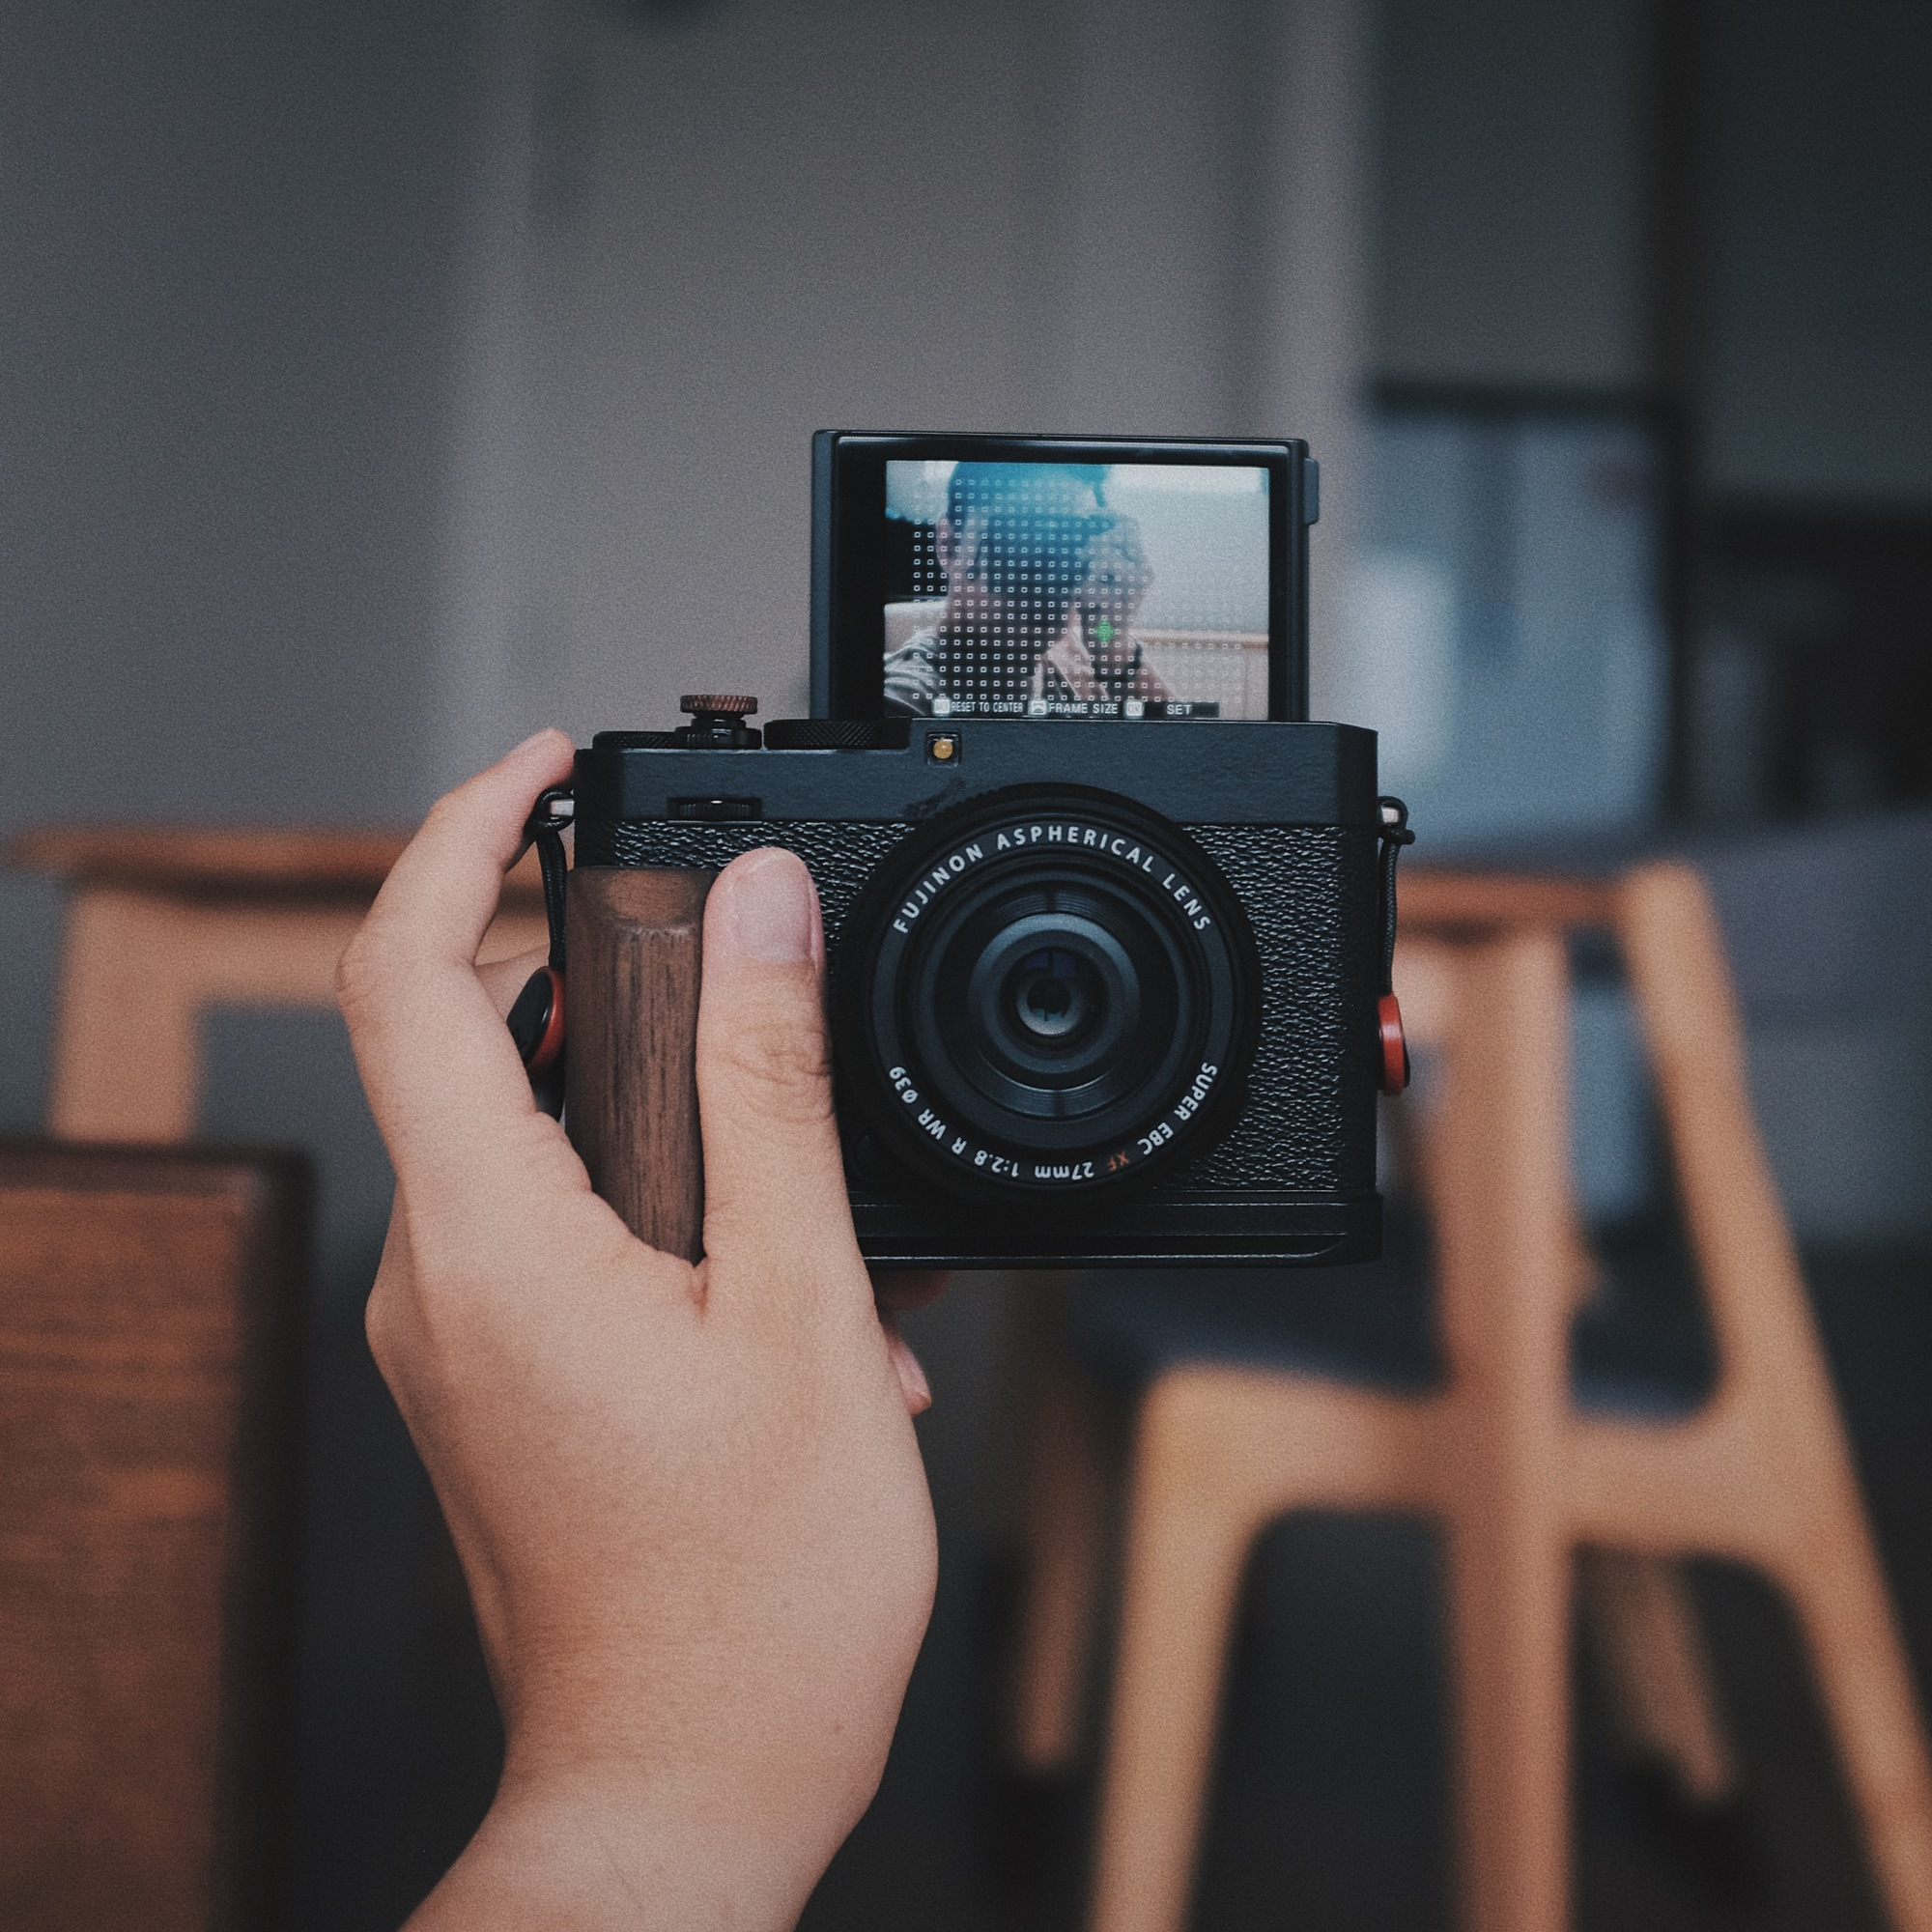
\includegraphics[width=\linewidth]{\envfinaldir/coverpic-prod.jpg}\par
            % \vskip 30pt
            \vfill

            \normalsize\rmfamily\scshape
            \copyright{} The Web Digest Project \hfill\large \envdatestr
        \end{center}
    \end{titlepage}
    % \restoregeometry
}
\newcommand{\simplehref}[1]{%
    \textcolor{blue!80!green}{\href{#1}{#1}}%
}
\renewcommand{\contentsname}{\center\Huge\sffamily\bfseries Contents\par\vskip 20pt}
\newcounter{ipartcounter}
\setcounter{ipartcounter}{0}
\newcommand{\ipart}[1]{
    % \vskip 20pt
    \clearpage
    \stepcounter{ipartcounter}
    \phantomsection
    \addcontentsline{toc}{chapter}{#1}
    % \begin{center}
    %     \Huge
    %     \sffamily\bfseries
    %     #1
    % \end{center}
    % \vskip 20pt plus 7pt
}
\newcounter{ichaptercounter}
\setcounter{ichaptercounter}{0}
\newcommand{\ichapter}[1]{
    % \vskip 20pt
    \clearpage
    \stepcounter{ichaptercounter}
    \phantomsection
    \addcontentsline{toc}{section}{\numberline{\arabic{ichaptercounter}}#1}
    \begin{center}
        \Huge
        \sffamily\bfseries
        #1
    \end{center}
    \vskip 20pt plus 7pt
}
\newcommand{\entrytitlefont}[1]{\subsection*{\raggedright\Large\sffamily\bfseries#1}}
\newcommand{\entryitemGeneric}[2]{
    % argv: title, url
    \parbox{\linewidth}{
        \entrytitlefont{#1}\par\vskip 5pt
        \footnotesize\ttfamily\mdseries
        \simplehref{#2}
    }\vskip 11pt plus 11pt minus 1pt
}
\newcommand{\entryitemGithub}[3]{
    % argv: title, url, desc
    \parbox{\linewidth}{
        \entrytitlefont{#1}\par\vskip 5pt
        \footnotesize\ttfamily\mdseries
        \simplehref{#2}\par\vskip 5pt
        \small\rmfamily\mdseries#3
    }\vskip 11pt plus 11pt minus 1pt
}
\newcommand{\entryitemAp}[3]{
    % argv: title, url, desc
    \parbox{\linewidth}{
        \entrytitlefont{#1}\par\vskip 5pt
        \footnotesize\ttfamily\mdseries
        \simplehref{#2}\par\vskip 5pt
        \small\rmfamily\mdseries#3
    }\vskip 11pt plus 11pt minus 1pt
}
\newcommand{\entryitemHackernews}[3]{
    % argv: title, hnurl, rawurl
    % \parbox{\linewidth}{
    %     \entrytitlefont{#1}\par\vskip 5pt
    %     \footnotesize\ttfamily\mdseries
    %     \simplehref{#3}\par
    %     \textcolor{black!50}{\href{#2}{#2}}
    % }\vskip 11pt plus 11pt minus 1pt
    \begin{minipage}{\linewidth}
            \entrytitlefont{#1}\par\vskip 5pt
            \footnotesize\ttfamily\mdseries
            \simplehref{#3}\par
            \textcolor{black!50}{\href{#2}{#2}}
    \end{minipage}\par\vskip 11pt plus 11pt minus 1pt
}







\begin{document}

\makeheader

\tableofcontents\clearpage




\ipart{Developers}
\ichapter{Hacker News}
\entryitemTwoLinks{Llama 4 Now Live on Groq}{https://news.ycombinator.com/item?id=43596470}{https://groq.com/llama-4-now-live-on-groq-build-fast-at-the-lowest-cost-without-compromise/}

\entryitemTwoLinks{The Llama 4 herd}{https://news.ycombinator.com/item?id=43595585}{https://ai.meta.com/blog/llama-4-multimodal-intelligence/}

\entryitemTwoLinks{What If We Made Advertising Illegal?}{https://news.ycombinator.com/item?id=43595269}{https://simone.org/advertising/}

\entryitemTwoLinks{Exeter's unassuming co-op worker leads double life as 'Lord of the Logos'}{https://news.ycombinator.com/item?id=43594396}{https://www.devonlive.com/whats-on/whats-on-news/exeters-unassuming-co-op-worker-10039941}

\entryitemTwoLinks{Show HN: I built a word game. My mom thinks it's great. What do you think?}{https://news.ycombinator.com/item?id=43593789}{https://www.whatsit.today/}

\entryitemTwoLinks{A Vision for WebAssembly Support in Swift}{https://news.ycombinator.com/item?id=43593596}{https://forums.swift.org/t/pitch-a-vision-for-webassembly-support-in-swift/79060}

\entryitemTwoLinks{Compilers: Incrementally and Extensibly (2024)}{https://news.ycombinator.com/item?id=43593088}{https://okmij.org/ftp/tagless-final/Compiler/index.html}

\entryitemTwoLinks{Earth's clouds are shrinking, boosting global warming}{https://news.ycombinator.com/item?id=43592756}{https://www.science.org/content/article/earth-s-clouds-are-shrinking-boosting-global-warming}

\entryitemTwoLinks{Europe needs its own social media platforms to safeguard sovereignty}{https://news.ycombinator.com/item?id=43592454}{https://mediascope.group/europe-needs-its-own-social-media-platforms-to-safeguard-sovereignty/}

\entryitemTwoLinks{Emulating an iPhone in QEMU}{https://news.ycombinator.com/item?id=43592409}{https://eshard.com/posts/emulating-ios-14-with-qemu}

\entryitemTwoLinks{Nebula Sans}{https://news.ycombinator.com/item?id=43591225}{https://nebulasans.com/}

\entryitemTwoLinks{Recreating Daft Punk's Something About Us}{https://news.ycombinator.com/item?id=43591050}{https://thoughts-and-things.ghost.io/recreating-daft-punks-something-about-us/}

\entryitemTwoLinks{Show HN: OCR pipeline for ML training (tables, diagrams, math, multilingual)}{https://news.ycombinator.com/item?id=43590998}{https://github.com/ses4255/Versatile-OCR-Program}

\entryitemTwoLinks{Trump's Tariff Formula Makes No Economic Sense. It's Also Based on an Error}{https://news.ycombinator.com/item?id=43590421}{https://www.aei.org/economics/president-trumps-tariff-formula-makes-no-economic-sense-its-also-based-on-an-error/}

\entryitemTwoLinks{OpenVertebrate Presents a Database of 13,000 3D Scans of Specimens}{https://news.ycombinator.com/item?id=43589989}{https://www.openculture.com/2024/03/openvertebrate-presents-a-massive-database-of-13000-3d-scans-of-vertebrate-specimens.html}

\entryitemTwoLinks{Learn electricity and electronics fundamentals without taking a formal course}{https://news.ycombinator.com/item?id=43589776}{https://simonmonk.org/tyee7}

\entryitemTwoLinks{AT\&T Email-to-Text Gateway Service Ending June 17}{https://news.ycombinator.com/item?id=43589523}{https://www.att.com/support/article/wireless/KM1061254/}

\entryitemTwoLinks{Trump's Tariffs Wipe Out over \$6T on Wall Street in Epic Two-Day Rout}{https://news.ycombinator.com/item?id=43589231}{https://www.wsj.com/finance/stocks/u-s-stock-futures-fall-further-after-china-retaliates-against-trump-tariffs-3be33fa7}

\entryitemTwoLinks{Annotated Unix Magic Poster}{https://news.ycombinator.com/item?id=43589042}{https://unixmagic.net/}

\entryitemTwoLinks{The 'Judicial Black Hole' of El Salvador's Prisons Is a Warning for Americans}{https://news.ycombinator.com/item?id=43588970}{https://www.rollingstone.com/politics/politics-features/el-salvador-prisons-warning-americans-trump-1235309721/}\ichapter{Phoronix}
\entryitemGeneric{\hskip 0pt{}Linux 6.15 Crypto Subsystem Delivers Faster AES-CTR For AMD Zen 5 \& Other x86\_64 CPUs}{https://www.phoronix.com/news/Linux-6.15-Crypto}

\entryitemGeneric{\hskip 0pt{}RISC-V With Linux 6.15 Adds Support For BFloat16 "BF16" Instructions}{https://www.phoronix.com/news/Linux-6.15-RISC-V}

\entryitemGeneric{\hskip 0pt{}Debian APT 3.0 Stable Released With New Package Solver \& Refined Text UI}{https://www.phoronix.com/news/Debian-APT-3.0-Released}

\entryitemGeneric{\hskip 0pt{}Resources 1.8 Released As A Great System Resource Monitor For GNOME}{https://www.phoronix.com/news/Resources-1.8-Released}

\entryitemGeneric{\hskip 0pt{}LACT 0.7.3 Further Enhances This GPU Configuration \& Monitoring Tool}{https://www.phoronix.com/news/LACT-0.7.3-Released}

\entryitemGeneric{\hskip 0pt{}FEX 2504 Ships More Optimizations For Running x86\_64 Linux Binaries On ARM64}{https://www.phoronix.com/news/FEX-2504-Released}

\entryitemGeneric{\hskip 0pt{}Intel Open Image Denoise Adds Support For AMD RDNA4 \& NVIDIA Blackwell}{https://www.phoronix.com/news/Intel-Open-Image-Denoise-2.3.3}

\entryitemGeneric{\hskip 0pt{}KDE Plasma Lands More Crash Fixes This Week, Refines Its Crash Reporting Wizard}{https://www.phoronix.com/news/KDE-Refines-DrKonqi}

\entryitemGeneric{\hskip 0pt{}Wine 10.5 Brings Vulkan H.264 Video Decoding, Mono 10.0 \& Bluetooth Pairing}{https://www.phoronix.com/news/Wine-10.5-Released}\ichapter{Dribbble}
\entryitemGeneric{\hskip 0pt{}Educational Website on Space Pollution}{https://dribbble.com/shots/25860515-Educational-Website-on-Space-Pollution}

\entryitemGeneric{\hskip 0pt{}CRYSTAL PRT\_2 // Mobile Version}{https://dribbble.com/shots/25860264-CRYSTAL-PRT-2-Mobile-Version}

\entryitemGeneric{\hskip 0pt{}Going for Gold}{https://dribbble.com/shots/25861716-Going-for-Gold}

\entryitemGeneric{\hskip 0pt{}LA Kings Mexican Heritage Theme Night Art}{https://dribbble.com/shots/25862720-LA-Kings-Mexican-Heritage-Theme-Night-Art}

\entryitemGeneric{\hskip 0pt{}Atomiq Unused Logo Design}{https://dribbble.com/shots/25861903-Atomiq-Unused-Logo-Design}

\entryitemGeneric{\hskip 0pt{}Ship Logo Design - Boat, Shield, Star, Waves}{https://dribbble.com/shots/25854151-Ship-Logo-Design-Boat-Shield-Star-Waves}

\entryitemGeneric{\hskip 0pt{}Interactive Speed Slider}{https://dribbble.com/shots/25851176-Interactive-Speed-Slider}

\entryitemGeneric{\hskip 0pt{}Croc logo}{https://dribbble.com/shots/25852607-Croc-logo}

\entryitemGeneric{\hskip 0pt{}Abstract}{https://dribbble.com/shots/25853030-Abstract}

\entryitemGeneric{\hskip 0pt{}Logo Design Selection Q1 2025}{https://dribbble.com/shots/25852275-Logo-Design-Selection-Q1-2025}

\entryitemGeneric{\hskip 0pt{}Jot Landing Page, Website Design, business web site}{https://dribbble.com/shots/25843658-Jot-Landing-Page-Website-Design-business-web-site}

\entryitemGeneric{\hskip 0pt{}Cloud Lightning}{https://dribbble.com/shots/25852815-Cloud-Lightning}

\entryitemGeneric{\hskip 0pt{}ef monogram}{https://dribbble.com/shots/25847206-ef-monogram}

\entryitemGeneric{\hskip 0pt{}Helpfull - Logo Redesign}{https://dribbble.com/shots/25847828-Helpfull-Logo-Redesign}

\entryitemGeneric{\hskip 0pt{}Outrigger Marketing Logo}{https://dribbble.com/shots/25848681-Outrigger-Marketing-Logo}

\entryitemGeneric{\hskip 0pt{}Wayflow Logo Design - Letter W, Waves, Flow}{https://dribbble.com/shots/25847473-Wayflow-Logo-Design-Letter-W-Waves-Flow}

\entryitemGeneric{\hskip 0pt{}Letter G set}{https://dribbble.com/shots/25845864-Letter-G-set}

\entryitemGeneric{\hskip 0pt{}Vínföng Final Wordmark}{https://dribbble.com/shots/25848505-V-nf-ng-Final-Wordmark}

\entryitemGeneric{\hskip 0pt{}Let down your hair}{https://dribbble.com/shots/25844844-Let-down-your-hair}

\entryitemGeneric{\hskip 0pt{}Chat GPT 4 Branding Concept}{https://dribbble.com/shots/25844194-Chat-GPT-4-Branding-Concept}

\entryitemGeneric{\hskip 0pt{}Sustainable contribution selector: percentage picker}{https://dribbble.com/shots/25843734-Sustainable-contribution-selector-percentage-picker}

\entryitemGeneric{\hskip 0pt{}FG}{https://dribbble.com/shots/25842733-FG}

\entryitemGeneric{\hskip 0pt{}Kovre Winery Logo Exploration}{https://dribbble.com/shots/25844706-Kovre-Winery-Logo-Exploration}

\entryitemGeneric{\hskip 0pt{}Crypto Portfolio Dashboard}{https://dribbble.com/shots/25841268-Crypto-Portfolio-Dashboard}


\ipart{Developers~~~~(zh-Hans)}
\ichapter{Solidot}
\entryitemGeneric{\hskip 0pt{}细菌氧代谢出现时间早于地球大氧化事件 }{https://www.solidot.org/story?sid=80972}

\entryitemGeneric{\hskip 0pt{}空调驱动全球能源需求增长}{https://www.solidot.org/story?sid=80971}

\entryitemGeneric{\hskip 0pt{}倭黑猩猩声音具有与人类语言相似的组合性}{https://www.solidot.org/story?sid=80970}

\entryitemGeneric{\hskip 0pt{}为何 AV1 仍未普及?}{https://www.solidot.org/story?sid=80969}

\entryitemGeneric{\hskip 0pt{}英特尔和台积电达成初步协议合资运营芯片制造业务}{https://www.solidot.org/story?sid=80968}

\entryitemGeneric{\hskip 0pt{}朝鲜黑客如何窃取数以十亿美元的加密货币}{https://www.solidot.org/story?sid=80967}

\entryitemGeneric{\hskip 0pt{}美国 34 家比特币矿场的耗电量超过洛杉矶}{https://www.solidot.org/story?sid=80966}

\entryitemGeneric{\hskip 0pt{}小行星 2024 YR4 撞击月球概率上调至 3.8\%}{https://www.solidot.org/story?sid=80965}

\entryitemGeneric{\hskip 0pt{}盖茨以 PDF 形式发布了 Altair BASIC 源代码}{https://www.solidot.org/story?sid=80964}

\entryitemGeneric{\hskip 0pt{}美国富人的寿命低于欧洲富人}{https://www.solidot.org/story?sid=80963}

\entryitemGeneric{\hskip 0pt{}部分音乐享受能力或来自遗传}{https://www.solidot.org/story?sid=80962}

\entryitemGeneric{\hskip 0pt{}微软 CTO 预测五年内 95\% 的代码由 AI 生成}{https://www.solidot.org/story?sid=80961}

\entryitemGeneric{\hskip 0pt{}雄性果蝇饮酒能增加对雌性的吸引力}{https://www.solidot.org/story?sid=80960}

\entryitemGeneric{\hskip 0pt{}PorteuX 2.0 释出}{https://www.solidot.org/story?sid=80959}

\entryitemGeneric{\hskip 0pt{}维基基金会称 AI 爬虫导致带宽消耗增加五成}{https://www.solidot.org/story?sid=80958}

\entryitemGeneric{\hskip 0pt{}任天堂将第一方游戏售价提高到 70/80 美元}{https://www.solidot.org/story?sid=80957}\ichapter{V2EX}
\entryitemGeneric{\hskip 0pt{}[问与答] 在东京旅游买哪些型号的 iPhone 作为备用机性价比高?}{https://www.v2ex.com/t/1123480}

\entryitemGeneric{\hskip 0pt{}[程序员] 高德地图上的那些充电桩价格信息有 API 获取吗?}{https://www.v2ex.com/t/1123479}

\entryitemGeneric{\hskip 0pt{}[OpenAI] 求证一件事, chat gpt 真会封号??}{https://www.v2ex.com/t/1123477}

\entryitemGeneric{\hskip 0pt{}[问与答] 出狱满一年了!虽然前路漫漫,但是未来可期。}{https://www.v2ex.com/t/1123476}

\entryitemGeneric{\hskip 0pt{}[VPS] 用 cursor 半天时间写了一个 VPS 促销信息面板 前后端+管理面板}{https://www.v2ex.com/t/1123475}

\entryitemGeneric{\hskip 0pt{}[分享创造] [极简倒计时 App] 喜欢番茄时钟或者需要倒计时提醒工具的 V 友来交流下~}{https://www.v2ex.com/t/1123472}

\entryitemGeneric{\hskip 0pt{}[Planet] Planet 的网页客户端}{https://www.v2ex.com/t/1123470}

\entryitemGeneric{\hskip 0pt{}[问与答] 大佬们,求开源可部署的 CRM 系统,类似于理发店的系统这种,有会员管理、消费管理、充值管理等。}{https://www.v2ex.com/t/1123469}

\entryitemGeneric{\hskip 0pt{}[分享创造] AI 辅助用 Rust 重写了一个 subconverter 有感}{https://www.v2ex.com/t/1123463}

\entryitemGeneric{\hskip 0pt{}[程序员] cursor 0.48 版本怎么这么难用了}{https://www.v2ex.com/t/1123462}

\entryitemGeneric{\hskip 0pt{}[分享发现] Copilot 超级会员 \$39/mo}{https://www.v2ex.com/t/1123460}

\entryitemGeneric{\hskip 0pt{}[SSD] 怎么判断固态硬盘是快要坏了?有什么征兆么}{https://www.v2ex.com/t/1123459}

\entryitemGeneric{\hskip 0pt{}[OpenWrt] Openwrt 使用 openclash 和 passwall2 都无法解决 ollama 拉取模型走机场流量的问题。}{https://www.v2ex.com/t/1123458}

\entryitemGeneric{\hskip 0pt{}[问与答] ios 使用 loon mitm 去广告安全吗}{https://www.v2ex.com/t/1123457}

\entryitemGeneric{\hskip 0pt{}[酷工作] 出海内容电商 AI+SaaS 初创团队招 [Golang] 后端长期兼职}{https://www.v2ex.com/t/1123456}

\entryitemGeneric{\hskip 0pt{}[上海] 世博 8 号线 [杨思站] 招合租室友}{https://www.v2ex.com/t/1123455}

\entryitemGeneric{\hskip 0pt{}[问与答] 如何限制 google 的搜索结果的地区偏好为香港?比如开🇯🇵节点用 chatgpt,但此时 google 搜索结果很多日文的,体验不好}{https://www.v2ex.com/t/1123454}

\entryitemGeneric{\hskip 0pt{}[程序员] 一个代理,又在本地跑,又在指纹浏览器跑 ytb, x,影响 ytb、x 的质量吗}{https://www.v2ex.com/t/1123452}

\entryitemGeneric{\hskip 0pt{}[职场话题] 怎么评估团队需要多少人}{https://www.v2ex.com/t/1123451}

\entryitemGeneric{\hskip 0pt{}[问与答] 有人买过 gemini 会员的吗?会员一天或者一个月可以用多少次 2.5pro}{https://www.v2ex.com/t/1123450}

\entryitemGeneric{\hskip 0pt{}[问与答] 有使用 Dell U2723qx 显示器的 V 友进来看下,问些问题}{https://www.v2ex.com/t/1123449}

\entryitemGeneric{\hskip 0pt{}[推广] 限时免费招募 AI-API 代理合作伙伴~~无需技术背景,一站式服务,技术问题我们全包}{https://www.v2ex.com/t/1123448}

\entryitemGeneric{\hskip 0pt{}[问与答] 按照 stackoverflow 教程执行 pg\_resetwal, postgresql 的数据库被清空了}{https://www.v2ex.com/t/1123446}

\entryitemGeneric{\hskip 0pt{}[Pixel] pixel 4 的人脸解锁问题无解了吗?}{https://www.v2ex.com/t/1123445}

\entryitemGeneric{\hskip 0pt{}[问与答] Windows 电脑发出不明通知声音,有大佬知道这是什么应用的通知声吗?}{https://www.v2ex.com/t/1123444}

\entryitemGeneric{\hskip 0pt{}[分享创造] 黄历✖️MCP 能发生点什么}{https://www.v2ex.com/t/1123443}

\entryitemGeneric{\hskip 0pt{}[分享创造] ReFormX-动态表单}{https://www.v2ex.com/t/1123442}

\entryitemGeneric{\hskip 0pt{}[Apple] 火箭有什么可靠的去广告规则吗}{https://www.v2ex.com/t/1123440}

\entryitemGeneric{\hskip 0pt{}[问与答] 三星 970 SSD 似乎有问题,求推荐硬盘}{https://www.v2ex.com/t/1123439}

\entryitemGeneric{\hskip 0pt{}[macOS] 8g Mac 怎么设置能恢复旧系统流畅度}{https://www.v2ex.com/t/1123438}

\entryitemGeneric{\hskip 0pt{}[问与答] 有大佬分析下秘塔搜索的``生成互动网页''是怎么实现的吗?}{https://www.v2ex.com/t/1123437}

\entryitemGeneric{\hskip 0pt{}[程序员] 关于在 Windows 端本地微调 Qwen 模型}{https://www.v2ex.com/t/1123436}

\entryitemGeneric{\hskip 0pt{}[推广] DMIT- PVM.LAX.Pro.\$49.9 \& \$100-三网优化 CN2GIA}{https://www.v2ex.com/t/1123435}

\entryitemGeneric{\hskip 0pt{}[分享发现] 京东全球购真的是个老鼠窝哈,包括自营的}{https://www.v2ex.com/t/1123433}

\entryitemGeneric{\hskip 0pt{}[macOS] macos Sequoia 15.4 Find My 查找里面看不到 Macbook Pro}{https://www.v2ex.com/t/1123432}

\entryitemGeneric{\hskip 0pt{}[媒体] jellyfin 把花絮识别成了正片}{https://www.v2ex.com/t/1123429}

\entryitemGeneric{\hskip 0pt{}[程序员] ai 和中医很像,突然的想法水一下。}{https://www.v2ex.com/t/1123428}

\entryitemGeneric{\hskip 0pt{}[MacBook] 毕业一年半 值得花 2 万买台 MacBook Pro 吗}{https://www.v2ex.com/t/1123427}

\entryitemGeneric{\hskip 0pt{}[Firefox] 分享一个 Firefox 用户主题 mimicfox userChrome.css}{https://www.v2ex.com/t/1123426}

\entryitemGeneric{\hskip 0pt{}[香港] 下周准备香港,开香港银行请教下}{https://www.v2ex.com/t/1123424}

\entryitemGeneric{\hskip 0pt{}[问与答] 现在还有什么不和谐资源的网盘,可以白嫖 1T 以上的存储空间吗}{https://www.v2ex.com/t/1123422}

\entryitemGeneric{\hskip 0pt{}[Apple] iPhone 这个 iCloud 云备份是不是默认只能 Wi-Fi 备份?}{https://www.v2ex.com/t/1123421}

\entryitemGeneric{\hskip 0pt{}[投资] 玩虚拟币合约,控制好仓位和强平价格,还会有什么其他风险?}{https://www.v2ex.com/t/1123419}

\entryitemGeneric{\hskip 0pt{}[问与答] 求推荐 magnet 链接批量分组下载办法}{https://www.v2ex.com/t/1123418}

\entryitemGeneric{\hskip 0pt{}[程序员] 远程全栈工作}{https://www.v2ex.com/t/1123417}

\entryitemGeneric{\hskip 0pt{}[程序员] cloudflare 开启小云朵就不能访问了这是为什么}{https://www.v2ex.com/t/1123416}

\entryitemGeneric{\hskip 0pt{}[OpenWrt] 解决 i226-V 由于「Detected Tx Unit Hang」错误导致的断网问题}{https://www.v2ex.com/t/1123415}

\entryitemGeneric{\hskip 0pt{}[JetBrains] gateway 是真的垃圾,我就想远程编辑远程文件这么难吗?}{https://www.v2ex.com/t/1123414}

\entryitemGeneric{\hskip 0pt{}[问与答] 去求职香港工作要注意什么?}{https://www.v2ex.com/t/1123413}

\entryitemGeneric{\hskip 0pt{}[上海] 浦东牡丹园好多吸游烟的}{https://www.v2ex.com/t/1123412}


\ipart{Generic News}
\ichapter{AP News}
\entryitemWithDescription{\hskip 0pt{}Sean `Diddy' Combs hit with new sex trafficking charges a month before trial}{https://apnews.com/article/79604824c58a007dd2f01a295ea8fab4}{}

\entryitemWithDescription{\hskip 0pt{}Microsoft employees protest at 50th anniversary party over Israel contract}{https://apnews.com/article/fadcb37bcce7e067f896ec5502d187b6}{}

\entryitemWithDescription{\hskip 0pt{}China hit brakes on TikTok deal after Trump announced wide-ranging tariffs, AP source says}{https://apnews.com/article/665e46fd5bb555e97c4d7301e07230df}{}

\entryitemWithDescription{\hskip 0pt{}An Oklahoma man has been charged with murder in the fatal shooting of a beloved Kansas priest}{https://apnews.com/article/f418a0f3933baaef73b359e32abd8363}{}

\entryitemWithDescription{\hskip 0pt{}AI vs. pro gambler's \$1 million March Madness bet coming down to Duke and Houston}{https://apnews.com/article/84d3e01d1f6ddff19c3af681f9ff681d}{}

\entryitemWithDescription{\hskip 0pt{}`Time to say goodbye': Kevin De Bruyne to leave Man City}{https://apnews.com/article/6b9b3b35c023b4c2e5c0a1efa760b277}{}

\entryitemWithDescription{\hskip 0pt{}In Tunisia, snails inch toward replacing red meat as people turn to cheaper protein}{https://apnews.com/article/b49a7582850be25702fbf47acf6b4375}{}

\entryitemWithDescription{\hskip 0pt{}Bodega cats make New Yorkers' hearts purr, even if they violate state regulations}{https://apnews.com/article/ebc2b1324c52bdbe6be70fcb71d12216}{}

\entryitemWithDescription{\hskip 0pt{}US bans government personnel in China from romantic or sexual relations with Chinese citizens}{https://apnews.com/article/c077ef57b0f7ae43dd0db41bea92238b}{}

\entryitemWithDescription{\hskip 0pt{}We got a behind-the-scenes look at Nintendo Switch 2. These are our thoughts}{https://apnews.com/article/63b0e49951ed09a9532ca55b4b35002e}{}

\entryitemWithDescription{\hskip 0pt{}Bye-bye, Helene, Milton and Beryl. Names from those nasty hurricanes are now retired}{https://apnews.com/article/57d1c2f83d8494d4a531479c638bd844}{}

\entryitemWithDescription{\hskip 0pt{}At 89, Fred Costello plays the organ on opening day in Rochester just like he has since 1977}{https://apnews.com/article/bf234264a40eb3d6fd1fd6103045379f}{}

\entryitemWithDescription{\hskip 0pt{}Athletics bat boy Stewart Thalblum takes down drone in left field}{https://apnews.com/article/e66410d8dd32a7fc69a31513d05fef43}{}






\clearpage
\leavevmode\vfill
\footnotesize

Copyright \copyright{} 2023-2025 Neruthes and other contributors.

This document is published with CC BY-NC-ND 4.0 license.

The entries listed in this newsletter may be copyrighted by their respective creators.

This newsletter is generated by the Web Digest project.

The newsletters are also delivered via Telegram channel \CJKunderline{\href{https://t.me/webdigestchannel}{https://t.me/webdigestchannel}}.\\
RSS feed is available at \CJKunderline{\href{https://webdigest.pages.dev/rss.xml}{https://webdigest.pages.dev/rss.xml}}.

This newsletter is available in PDF at
\CJKunderline{\href{https://webdigest.pages.dev/}{https://webdigest.pages.dev/}}.

The source code being used to generate this newsletter is available at\\
\CJKunderline{\href{https://github.com/neruthes/webdigest}{https://github.com/neruthes/webdigest}}.

This newsletter is also available in
\CJKunderline{\href{http://webdigest.pages.dev/readhtml/\envyear/WebDigest-20250406.html}{HTML}} and
\CJKunderline{\href{https://github.com/neruthes/webdigest/blob/master/markdown/\envyear/WebDigest-20250406.md}{Markdown}}.


\coverpic{https://unsplash.com/photos/an-aerial-view-of-a-sandy-beach-and-ocean-i38Wgx6RRN0}{saeed ghavam shahidi}


\end{document}
